\textbf{Name:} \\

\medskip

\textbf{Conspirators:} 

\medskip
\medskip

\hrule

\medskip


\assignmentsonly{\pleasesubmitprojectdraft}



\begin{enumerate}

  \item (3 + 3 + 3)

  \textit{Highly Optimized Tolerance:}

  This question is based on Carlson and Doyle's 1999 paper
  ``Highly optimized tolerance: {A} mechanism for power
  laws in design systems''~\cite{carlson1999a}.
  In class, we made our way through a discrete version
  of a toy HOT model of forest fires.
  This paper revolves around the equivalent continuous model's
  derivation.
  You do not have to perform the derivation but rather
  carry out some manipulations of probability distributions
  using their main formula.

  Our interest is in Table I on p.\ 1415:
  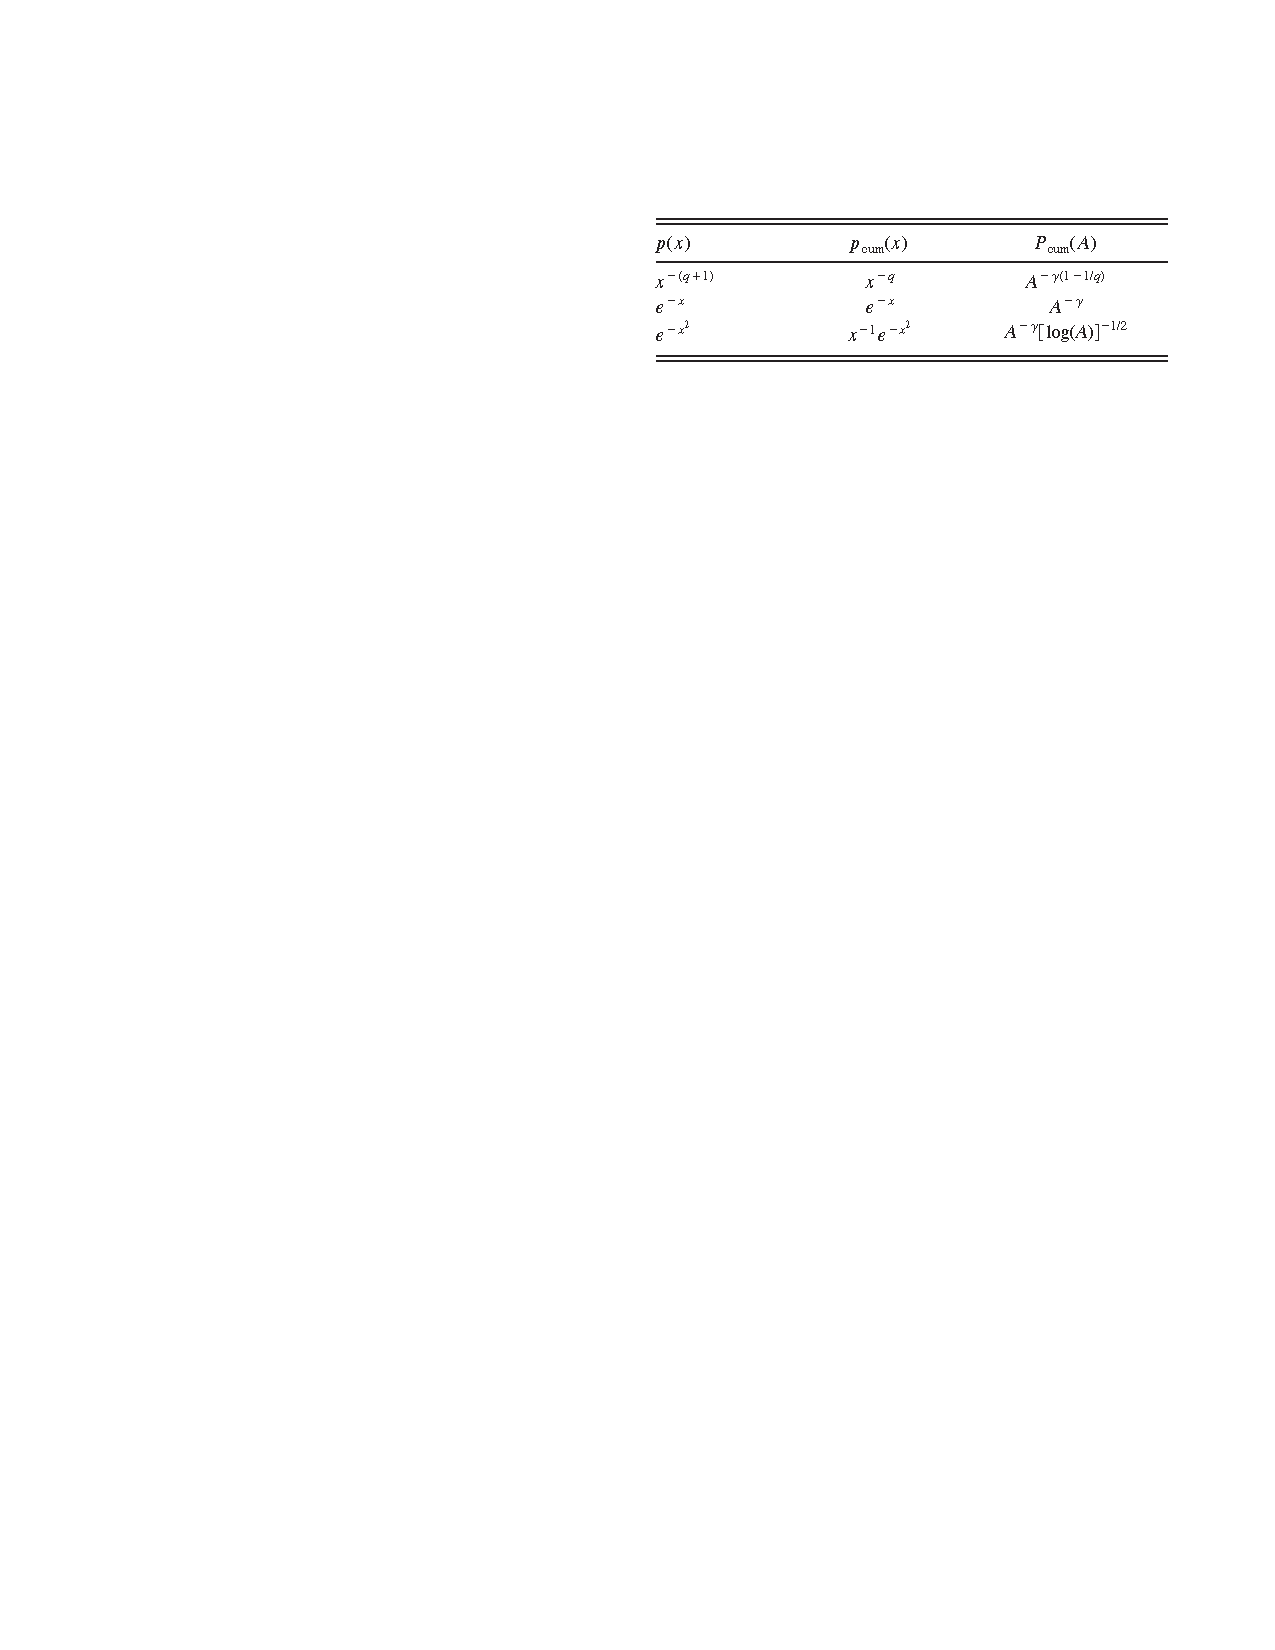
\includegraphics[width=0.7\textwidth]{carlson1999a_tab1.pdf}\\
  and Equation 8 on the same page:
  $$
  P_{\ge}(A)
  =
  \int_{p^{-1}(A^{-\gamma})}^{\infty}
  p(\mathbf{x})
  \dee{\mathbf{x}}
  =
  p_{\ge}
  \left(
    p^{-1}
    \left(
      A^{-\gamma}
    \right)
  \right),
  $$
  where $\gamma = \alpha + 1/\beta$
  and we'll write $P_{\ge}$ for $P_{\rm cum}$.

  Please note that $P_{\ge}(A)$
  for $x^{-(q+1)}$ is not correct.
  Find the right one!

  Here, $A(\mathbf{x})$ is the area connected 
  to the point $\mathbf{x}$ (think connected patch of trees for forest fires).
  The cost of a `failure' (e.g., lightning) beginning at $\mathbf{x}$
  scales as $A(\mathbf{x})^{\alpha}$
  which in turn occurs with probability 
  $p(\mathbf{x})$.  
  The function $p^{-1}$ is the inverse function of $p$.

  Resources associated with point $\mathbf{x}$ 
  are denoted as $R(\mathbf{x})$ and area is
  assumed to scale with resource as
  $A(\mathbf{x}) \sim R^{-\beta}(\mathbf{x})$.

  Finally, $p_{\ge}$ is the complementary cumulative
  distribution function for $p$.

  As per the table, determine
  $p_{\ge}(x)$
  and
  $P_{\ge}(A)$
  for the following (3 pts each):
  \begin{enumerate}
  \item
    $
    p(x) = c x^{-(q+1)}$,
  \item
    $
    p(x) = c e^{-x}$, and 
  \item
    $
    p(x) = c e^{-x^2}.
    $
  \end{enumerate}

  Note that these forms are for the tails of $p$ only,
  and you should incorporate a constant
  of proportionality $c$, which is not shown
  in the paper.

  
   \solutionstart

   %% solution goes here

   \solutionend

    \item
      The discrete version of HOT theory:

      From lectures, we had the following.

      Cost: Expected size of `fire' in a $d$-dimensional lattice:
      $$
      C_{\rm fire}
      \propto \sum_{i=1}^{N_{\rm sites}} p_i a_i
      $$ 
      where 
      $a_i$ = area of $i$th site's region,
      and
      $p_i$ = avg.\ prob.\ of fire at site $i$ over a given time period.

      The constraint for building and maintaining 
      $(d-1)$-dimensional firewalls in $d$-dimensions is
      $$
      C_{\rm firewalls} 
      \propto 
      \sum_{i=1}^{N_{\rm sites}} a_i^{(d-1)/d} a_i^{-1},
      $$
      where we are assuming isometry.

      Using Lagrange Multipliers, and, optionally, safety goggles,
      rubber gloves, a pair of tongs, and a maniacal laugh,
      determine that:
      $$ 
      p_i 
      \propto 
      a_i^{-\gamma} 
      = 
      a_i^{-(1 + 1/d)}.
      $$

      %%  and therefore that 
      %%  $$
      %%  \Prob(a_i) 
      %%  \propto 
      %%  a_i^{-\gamma}.
      %%  $$

      
   \solutionstart

   %% solution goes here

   \solutionend


\item (3 + 3 + 3 + 3)

  A courageous coding festival:

  Code up the discrete HOT model in 2-$d$.
  Let's see if we find any of these super-duper power laws
  everyone keeps talking about.  We'll follow the same
  approach as the $N$ = $L$$\times$$L$ 2-$d$ forest discussed in lectures.

  Main goal: extract yield curves as a function
  of the design $D$ parameter as described below.

  Suggested simulations elements:
  \begin{itemize}
  \item 
    Take $L=32$ as a start.  Once your code is running, see if $L=64$, 128, or more might
    be possible.
    (The original sets of papers used all three of these values.)
    Use a value of $L$ that's sufficiently large to produced useful
    statistics but not prohibitively time consuming for simulations.
  \item 
    Start with no trees.
  \item 
    Probability of a spark at the $(i,j)$th site:
    $
    P(i,j) \propto e^{-i/\ell} e^{-j/\ell}
    $
    where $(i,j)$ is tree position with the indices
    starting in the top left corner ($i,j=1$ to $L$).
    (You will need to normalize this properly.)
    The quantity $\ell$ is the characteristic
    scale for this distribution.
    Try out $\ell = L/10$.
  \item 
    Consider a design problem of $D=1$, $2$, $L$, and $L^{2}$.
    (If $L$ and $L^{2}$ are too much, you can drop them.
    Perhaps sneak out to $D=3$.)
    Recall that the design problem is to test $D$ randomly
    chosen placements of the next tree against the
    spark distribution.
  \item 
    For each test tree, 
    compute the average forest fire size over the full spark
    distribution: 
    $$
    \sum_{i,j} P(i,j) S(i,j),
    $$
    where $S(i,j)$ is the size of the forest component
    at $(i,j)$.
    Select the tree location with the highest average yield and plant a tree there.
  \item 
    Add trees until the 2-$d$ forest is full, measuring average yield as a function of trees added.
  \item 
    Only trees within the cluster surrounding the ignited tree burn
    (trees are connected through four nearest neighbors).
  \end{itemize}

  \begin{enumerate}
  \item 
    Plot the forest at (approximate) peak yield.
  \item 
    Plot the yield curves for each value of $D$,
    and identify (approximately) the peak yield and the density
    for which peak yield occurs for each value of $D$.
  \item 
    Plot Zipf (or size) distributions of tree component sizes $S$
    at peak yield.
    Note: You will have to rebuild forests
    and stop at the peak yield value of $D$ to
    find these distributions.
    By recording the sequence of optimal tree planting,
    this can be done without running the simulation again.
  \item
    Extra level: Plot Zipf (or size) distributions for $D=L^2$ for
    varying tree densities $\rho=0.10, 0.20, \ldots, 0.90$.
    This will be an effort to reproduce
    Fig.~3b in~\cite{carlson2000a}.
  \end{enumerate}

  Hint: 
  Working on un-treed locations will
  make choosing the next location easier.  

  
   \solutionstart

   %% solution goes here

   \solutionend




\end{enumerate}
